
\chapter{Downloading and Reading the Data}
\label{sec:download}
There are two main components to the EISPAC software: (1) a set of command line scripts and (2) the
Python package itself. In this chapter we will give a very brief overview of how to read and explore
the EIS data contained in the level-1 HDF5 files. The next chapter covers how to fit the data with Gaussian functions.

\section{Using the command line scripts}
The command line scripts should be automatically installed and registered with the OS as part of
installing EISPAC. These scripts are designed to help users quickly browse, download, and fit Gaussian functions to the data. To use a script, simply enter its name in the command line from any directory in which you have read and write privileges. \marginnote{\textbf{Note well:} some scripts will default to saving files to your current working directory, therefore we recommend running the scripts from the directory in which you intend to do most of your analysis.}

There are currently four command line scripts available,

\begin{itemize}
\item[\bf eis\_catalog -] GUI tool from searching the as-run EIS data catalog and downloading the HDF5 files your computer. Can also generate a text list of files to download.

\item[\bf eis\_browse\_templates -] GUI tool for browsing the fit templates corresponding to each spectral window in a given observation set and copying the template files from EISPAC to your current working directory (fit templates are explained more in the next chapter)

\item[\bf eis\_download\_files -] Command line tool for downloading a the level-1 HDF5 files assoiated with one or more level-0 EIS fits files. Can also download an entire list of files using the text output of \verb+eis_catalog+. Example usage,
\begin{lstlisting}
>>> eis_downdload_files eis_l0_20190404_131513.fits
\end{lstlisting}

\item[\bf eis\_fit\_files -] Command line tool for fitting all of the HDF5 files in a given directory with each fit template found in another directory. Example usage,
\begin{lstlisting}
>>> eis_fit_files ./eis_study/ ./eis_study/templates/
\end{lstlisting}
\end{itemize}

\section{Reading and Exploring data with EISPAC}
Once installed, EISPAC can be imported into any Python script or interactive session with a simple \verb+import eispac+ statement. Assuming you have already downloaded some data, the following code snippet below illustrates how to how to read the level-1 data from the spectral window containing the
\ion{Fe}{12} 195.12\,\AA line (window 7, in our example file). At the end of the chapter we will show how to examine a data header file to determine what wavelengths are available in a given observation.

\begin{lstlisting}[language=Python]
>>> import eispac
>>> data_filename = 'eis_20190404_131513.data.h5'
>>> data_cube = eispac.read_cube(data_filename, 195.12)
\end{lstlisting}

The \verb+read_cube()+ function will read and apply all of the calibration and pointing corrections
necessary for scientific analysis. The functions takes three arguments:
\begin{enumerate}
\item[\bf filename] (str or pathlib path) - Name or path of either the data or head HDF5 file for a
  single EIS observation
\item[\bf window] (int or float, optional) - Requested spectral window number (if <= 24) or the
  value of any wavelength within the requested window (in units of [Angstrom]). Default is "0"
\item[\bf apply\_radcal] (bool, optional) - If set to True, will apply the pre-flight radiometric
  calibration curve found in the HDF5 header file and set units to $erg/(cm^2 s sr)$. If set to False,
  will simply return the data in units of photon counts. Default is True.
\end{enumerate}

The return value is an \verb+EISCube+ class instance which contains calibrated intensities (or photon
counts), corrected wavelengths, and all of the associated metadata. \verb+EISCube+ objects are a
subclass of \verb+NDCube+ (from the Sunpy-affiliated package of the same name) and, as such, have
built-in slicing and coordinate conversion capabilities due to an accompanying World Coordinate
System (WCS) object. For example, you can slice an \verb+NDCube+ object using either array indices or
by inputting physical coordinates to the \verb+.crop_by_coords()+ method. Please see the
\verb+ndcube+ documentation\sidenote{\url{https://docs.sunpy.org/projects/ndcube/en/stable/index.html}} for more information about slicing and manipulating \verb+NDCube+ objects.

The \verb+EISCube+ subclass extends \verb+ndcube+ by including a few additional features.
First, an extra \verb+.wavelength+ attribute has been added which contains a 3D array
with the corrected wavelength values at all locations within the cube. This correction accounts for a
systematic spectral shift caused by a tilt in orientation of the in the EIS slit relative to the CCD.
Slicing an \verb+EISCube+ will also appropriately slice the wavelength array. Secondly, four methods
are included to quickly perform common EIS image processing,

\begin{itemize}
    \item The \verb+.apply_radcal()+ and \verb+.remove_radcal()+ methods can be used to convert the
    data and uncertainty values to and from intensity and photon count units using the pre-flight
    radiometric calibration curve provided in the HDF5 header file. Currently, neither method takes
    any arguments. Future versions of EISPAC will allow users to specific their own calibration curves.
    \item The \verb+.sum_spectra()+ method sums the data along the wavelength axis and returns a new, 2D \verb+NDCube+ with just the data (no uncertainty or wavelength information). It requires no arguments.
    \item The \verb+.smooth_cube()+ method applies a boxcar moving average to the data along one or more spatial axes. It requires a single argument, "width", that must be either a singular value or list of ints, floats, or astropy.units.Quantity instances specifying the number of pixels or angular distance to smooth over. If given a single value, only the y-axis will be smoothed. Floats and angular distances will be converted to the nearest whole pixel value. If a width value is even, width + 1 will be used instead. \verb+.smooth_cube()+ also accepts any number of optional keyword arguments that will be passed to the astropy.convolution.convolve()
    function, which does the actual smoothing operation.
\end{itemize}

The calibrated intensity and uncertainty values are stored in numpy arrays in the \verb+.data+ and \verb+.uncertainty+ attributes. The order of the axes are (slit position, raster step, wavelength) which correspond to the physical axes of (Solar-Y, Solar-X, Wavelength). You can inspect the dimensions of an \verb+NDCube+ object like so,

\begin{lstlisting}[language=Python]
>>> data_cube.dimensions
[512, 87, 24] pix
\end{lstlisting}

As you can see, our example data has dimensions of \verb+(512, 87, 24)+. That is, 512 pixels along the slit (in the Solar-Y direction), 87 raster steps in the X direction, and 24 pixels in the dispersion direction.

All metadata and information from the HDF5 header file are packed into a single dictionary stored in the \verb+.meta+ attribute of the \verb+EISCube+. The structure of the \verb+.meta+ dictionary mirrors the internal structure of the HDF5 file, with a few extra keys added for convenience. You can explore the contents with the usual Python commands,

\begin{lstlisting}[language=Python]
>>> data_cube.meta.keys()
dict_keys(['filename_data', 'filename_head', 'wininfo', 'iwin', 'iwin_str', 'index', 'pointing', 'wave', 'radcal', 'slit_width', 'slit_width_units', 'ccd_offset', 'wave_corr', 'wave_corr_t', 'wave_corr_tilt', 'date_obs', 'date_obs_format', 'duration', 'duration_units', 'aspect_ratio', 'notes'])
>>> data_cube.meta['pointing']['x_scale']
2.9952
>>> data_cube.meta['radcal']
array([8.06751  , 8.060929 , 8.054517 , 8.048271 , 8.042198 , 8.036295 ,
       8.030562 , 8.024157 , 8.017491 , 8.010971 , 8.0046015, 7.998385 ,
       7.9923196, 7.9864078, 7.980654 , 7.975055 , 7.969617 , 7.9643393,
       7.959224 , 7.9542727, 7.949487 , 7.9448686, 7.9404206, 7.9361415],
      dtype=float32)
\end{lstlisting}

Here \verb+x_scale+ is the number of arcsec per step in the raster. Most EIS rasters take more than
1 arcsec per step, which degrades the spatial resolution but increases the cadence. The variable
\verb+radcal+ is the pre-flight calibration curve for this data window. It includes all of the
factors for converting counts directly to erg cm$^{-2}$ s$^{-1}$ sr$^{-1}$.

We can make a quick image of the EIS data by making use of the \verb+.plot()+ method provided in all \verb+NDCube+ objects (note, it usually helps to sum along the dispersion direction first).

\begin{lstlisting}[language=Python]
>>> data_cube.sum_spectra().plot(aspect=data_cube.meta['aspect_ratio'])
\end{lstlisting}

\begin{marginfigure}
  \centerline{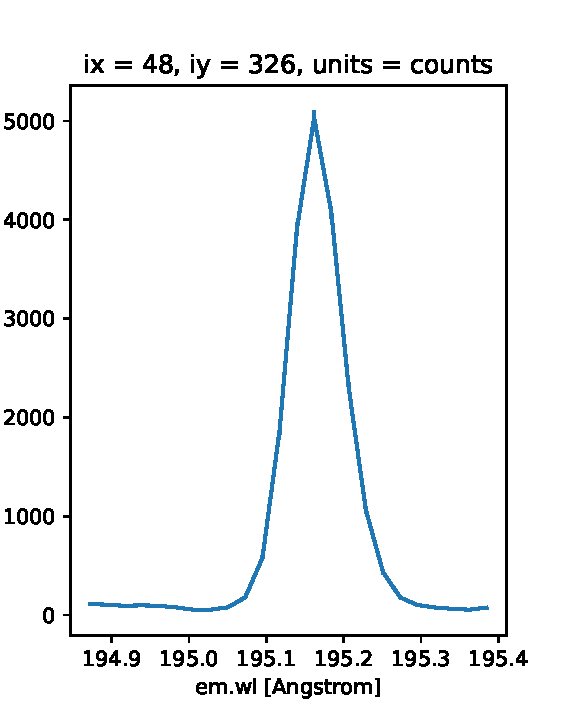
\includegraphics[clip,width=\linewidth]{figures/ex_spectrum.pdf}}
  \caption{An example \ion{Fe}{12} 195.119\,\AA\ line profile from the raster.}
  \label{fig:spectrum}
\end{marginfigure}

The \verb+.plot()+ method can also be used to display the spectrum from a single pixel, as shown
below. For illustration, we also convert the data back in units of photon counts (this is the same as
dividing the calibrated data by the \verb+.meta['radcal']+ array).

\begin{lstlisting}[language=Python]
>>> ix = 48
>>> iy = 326
>>> spec = data_cube[iy,ix,:].remove_radcal()
>>> spec_plot = spec.plot()
>>> spec_plot.set_title(f'ix = {ix}, iy = {iy}, units = counts')
\end{lstlisting}

To perform more advanced plotting, such as logarithmically scaling the intensities, you will need to extract the data from the \verb+EISCube+ and create the figure yourself using any of the various Python plotting libraries. For example,
\begin{marginfigure}
  \centerline{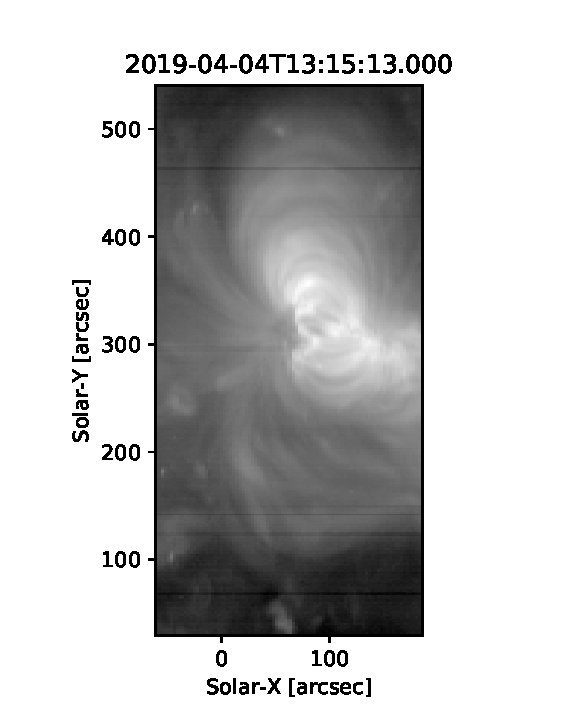
\includegraphics[clip,width=\linewidth]{figures/ex_log-scaled_raster.pdf}}
  \caption{An example image formed by summing the data for the \ion{Fe}{12} spectral window in the
    dispersion direction. In a subsequent chapter we'll discuss fitting the spectra.}
  \label{fig:raster}
\end{marginfigure}
\marginnote{\textbf{Plotting tip:} setting both "aspect" (y\_scale/x\_scale) and "extent" (data range as [left, right, bottom, top]) in \texttt{plt.imshow()} can sometimes give unexpected results. You may need to experiment with the combination of keywords needed to get the plot you expect.}

\begin{lstlisting}[language=Python]
import numpy as np
import matplotlib.pyplot as plt

raster_sum = np.sum(data_cube.data, axis=2) # or data_cube.sum_spectra().data
scaled_img = np.log10(raster_sum)

plt.figure()
plt.imshow(scaled_img, origin='lower', extent=data_cube.meta['extent_arcsec'], cmap='gray')
plt.title(data_cube.meta['date_obs'][-1])
plt.xlabel('Solar-X [arcsec]')
plt.ylabel('Solar-Y [arcsec]')
plt.show()
\end{lstlisting}

We usually don't care about the numbering of the data windows. It's more natural to want to read
the data corresponding to a particular wavelength. The \verb+eispac.read_wininfo()+ function can be used help identify the spectral contents of each data window. The function takes an input header file and returns a record array containing the window numbers, min and max wavelengths and primary spectral line for each data window. Note: for your convenience, a copy of the \verb+wininfo+ array is also stored in the \verb+EISCube.meta+ dictionary.
\begin{lstlisting}[language=Python]
>>> import eispac
>>> header_filename = 'eis_20190404_131513.head.h5'
>>> wininfo = eispac.read_wininfo(header_filename, 195.12)
>>> wininfo.dtype.names
('iwin', 'line_id', 'wvl_min', 'wvl_max', 'nl', 'xs')
>>> wininfo[0:4]
rec.array([(0, 'Fe XI 180.400', 180.03426, 180.72559, 32, 661),
           (1, 'Ca XV 182.100', 181.75139, 182.44266, 32, 738),
           (2, 'Fe X 184.720', 183.82512, 185.5865 , 80, 831),
           (3, 'Fe XII 186.750', 186.3891 , 187.0802 , 32, 946)],
          dtype=[('iwin', '<i4'), ('line_id', '<U64'), ('wvl_min', '<f4'),
                 ('wvl_max', '<f4'), ('nl', '<i4'), ('xs', '<i4')])
\end{lstlisting}
We can then use a numpy.where() call on the wininfo array to map wavelength to window number.
Users familiar with IDL may be interested to note that numpy record arrays can be accessed similarly to an IDL array of structures (e.g. instead of \verb+wininfo['wvl_min']+ below, you could also use \verb+wininfo.wvl_min+).
\begin{lstlisting}
>>> import numpy as np
>>> wvl = 195.119
>>> p = (wininfo['wvl_max'] - wvl)*(wvl - wininfo['wvl_min'])
>>> iwin = np.where(p >= 0)[0]
>>> iwin
array([7], dtype=int64)
\end{lstlisting}
If the result is an empty array, the wavelength is not in the data.
